\documentclass[10pt,twocolumn]{article} 
\usepackage{simpleConference}
\usepackage{times}
\usepackage{graphicx}
\usepackage{amssymb}
\usepackage{url,hyperref}

\hyphenation{op-tical net-works semi-conduc-tor}
\usepackage{listings}
\usepackage{color}

\definecolor{dkgreen}{rgb}{0,0.6,0}
\definecolor{gray}{rgb}{0.5,0.5,0.5}
\definecolor{mauve}{rgb}{0.58,0,0.82}

\lstset{frame=tb,
  language=Java,
  aboveskip=3mm,
  belowskip=3mm,
  showstringspaces=false,
  columns=flexible,
  basicstyle={\small\ttfamily},
  numbers=none,
  numberstyle=\tiny\color{gray},
  keywordstyle=\color{blue},
  commentstyle=\color{dkgreen},
  stringstyle=\color{mauve},
  breaklines=true,
  breakatwhitespace=true,
  tabsize=3
}


\begin{document}


\title{Tribune: An Externally Consistent Database Common Access API for the Global Data Plane}
\author{Matt Weber, Shiyun Huang and Lawrence Supian\\
Department of Electrical Engineering and Computer Sciences (EECS) \\
University of California, Berkeley\\
Email: matt.weber, jane.huang, lsupian@berkeley.edu
}

\maketitle
\thispagestyle{empty}


\begin{abstract}
	The Global Data Plane (GDP) is a distributed data storage system with the objective of providing persistent data storage to devices in the internet of things. The GDP has a variety of useful properties including data security, a flat namespace, and location independent routing, that improve the availability and efficiency of universal data storage. As a key component in the Terraswarm project and the SwarmOS, the GDP provides log based storage and routing between sensors and actuators embedded in the physical world. Logs are the fundamental primitive of the GDP, but some CAAPIs (a Common Access Application Programming Interface) require stronger semantics. In this paper we introduce Tribune, a multi-writer log CAAPI that enforces Google Spanner-like external consistency. We compare the trusted Paxos based replication scheme with attack tolerant Byzantine Agreement and evaluate optimistic concurrency against the lock table-based concurrency control scheme used by Google Spanner. In a performance evaluation we found the optimistic algorithm to be generally faster than the comparable lock table approach, particularly when paired with Byzantine agreement. Our long term goal is to provide PTIDES style deterministic execution semantics for swarmlets in the SwarmOS that choose to access time-aware multi-writer logs.
\end{abstract}

\section{Introduction}
The Internet of Things (IoT) presents a new paradigm for computer systems, enabling technologies like  context-aware apps, extensible cyber-physical systems, large scale sensor data collection for machine learning, and smart cities. But systems of the future will not come for free: engineers will need ubiquitous computing infrastructure in the form of platforms, services, and tools as a foundation for their work. The Terraswarm project \cite{lee_terraswarm_2012} seeks to address the gap between the development resources of today and those needed to engineer the coming swarm of interconnected devices \cite{rabaey_swarm_2011}. There are many dimensions of the problem to be considered, including verification tools, low-power sensors, programming models, and persistent universally available data storage. The last point in particular is of primary concern to swarmlet (an application in the swarm) developers who need data accessible across different usage modes and application contexts \cite{DabbeltKubiatowicz13_CaseForUniversalDataPlane}.

The Global Data Plane (GDP) \cite{Kubiatowicz14_EnablingSwarmThroughGlobalDataPlane} is a TerraSwarm project that seeks to extend upon the capabilities of the Cloud to meet the needs of decentralized and interoperable swarmlets. Oceanstore \cite{rhea_pond:_2003} provides a starting point, as data must be globally available, durable, private, secure, and efficiently accessible. Additionally, the GDP must support storage and distribution of streaming sensor data, which it achieves through log-based data storage in a flat address space. As such, the log is a principle component of the GDP, and could be used as the fundamental building block for arbitrarily complicated systems for information representation. This design choice does not limit the efficiency or expressiveness of the GDP, because the GDP supports a Common Access Application Programming Interface (CAPPI) for data representations with sophisticated semantics or complex structure.  Although possible, the process of reconstructing a full database or key-value store from log data would be prohibitively expensive if every time the sophisticated data structure were needed it had to be built from logs and then immediately thrown away. A CAAPI can maintain the current state of the enhanced structure  
directly and function as a sort of GDP cache for a particular data representation.

\begin{figure}[!b]
  \begin{center}
    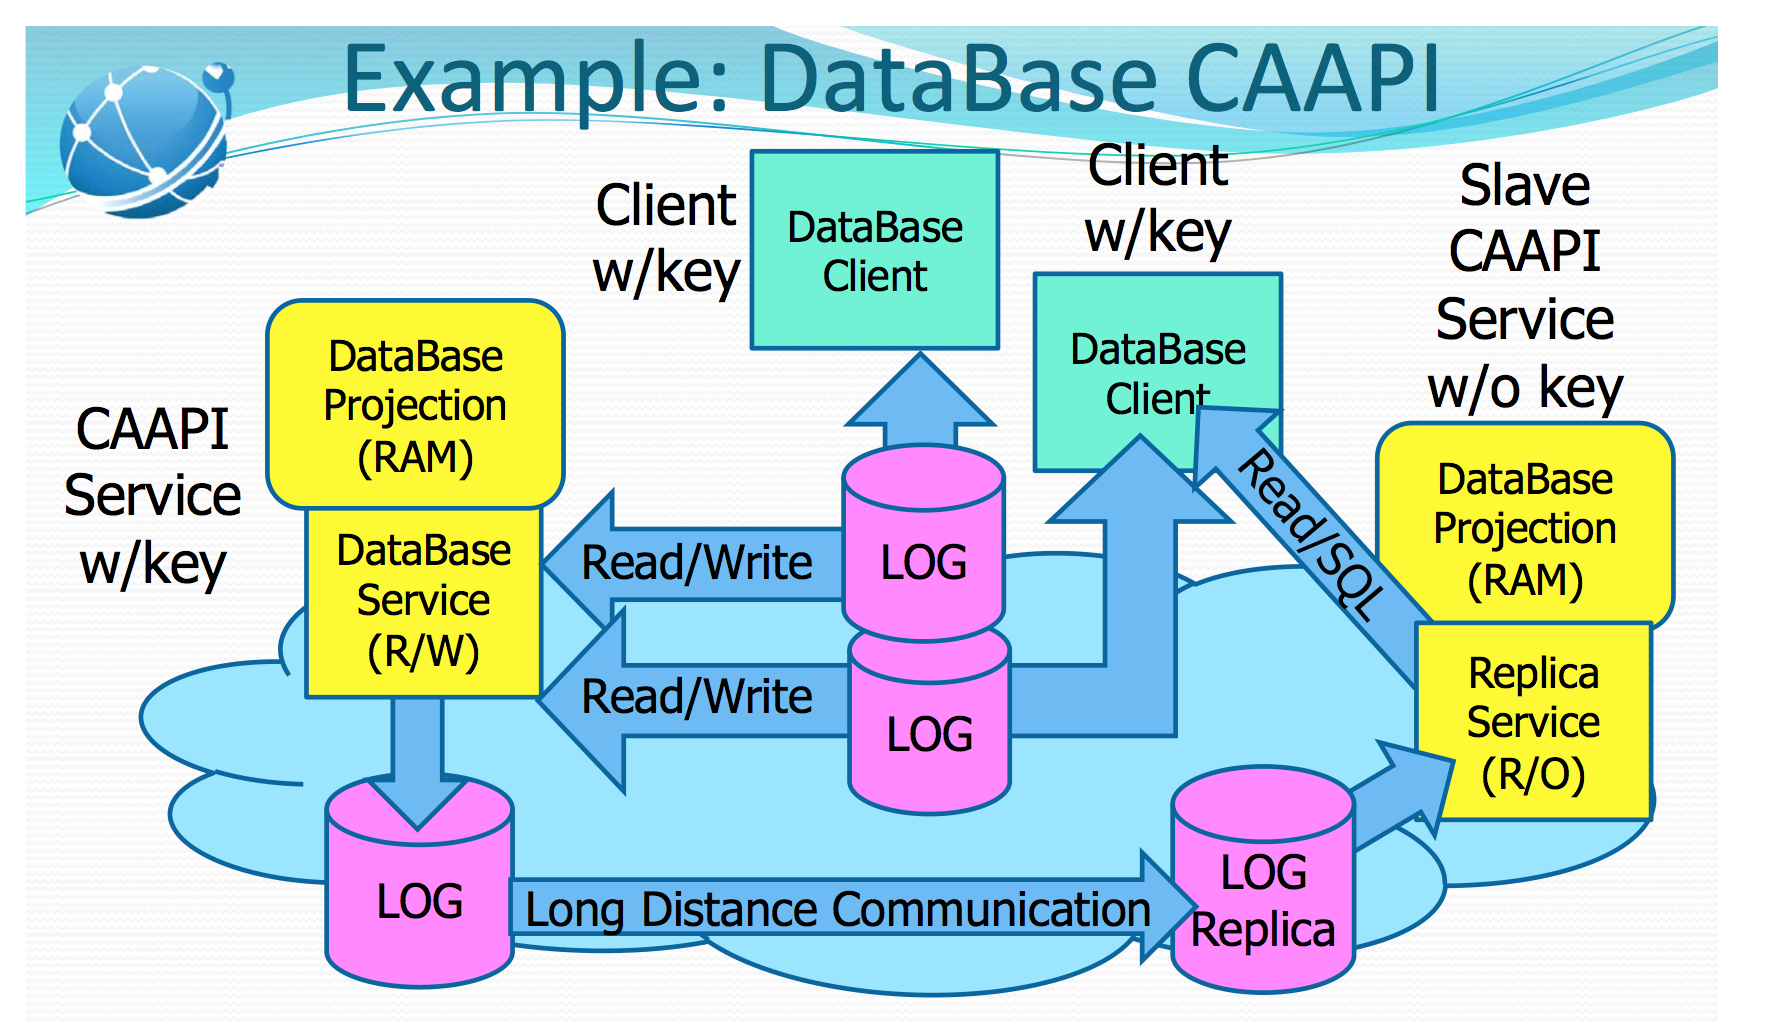
\includegraphics[width=3.5in]{Images/Database_CAAPI.png}
  \end{center}

  \caption{\small An illustration of a database CAAPI. Image from slide 17 of \cite{Kubiatowicz14_EnablingSwarmThroughGlobalDataPlane} }
  \label{Database_CAAPI}
\end{figure}

Although CAAPIs can be used in the GDP to store data efficiently, they also have the capacity to  enforce semantics on the behavior of operations on data. This work, Tribune, is an example of a CAAPI that enforces external consistency along with standard ACID semantics on the behavior of a multi-writer log. The general concept of this style of CAAPI is illustrated in Figure~\ref{Database_CAAPI}. Tribune's name is a reference to the role of an ancient Roman Tribune, an elected official with the power to intervene on behalf of the common people by vetoing legislation from the senate. In a similar respect, Tribune can control transactions that attempt to write to a protected log in this multi-writer merge style, and abort transactions that violate its semantics. 

This paper is organized as follows: Section II provides background information on the database behavior we seek to emulate in Tribune. Section III gives an overview of the system architecture and design. Section IV goes into the implementation details for our most interesting algorithms. Section V elaborates on our test environment setup and presents benchmark results. In Section VI we address the direction of future work. We conclude with Section VII.


\begin{figure}[!b]
  \begin{center}
    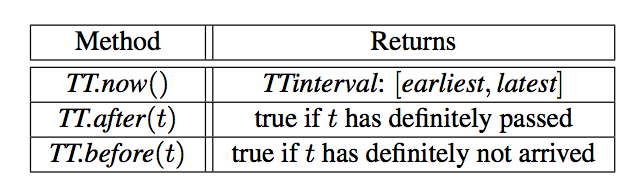
\includegraphics[width=3.5in]{Images/TrueTime.png}
% 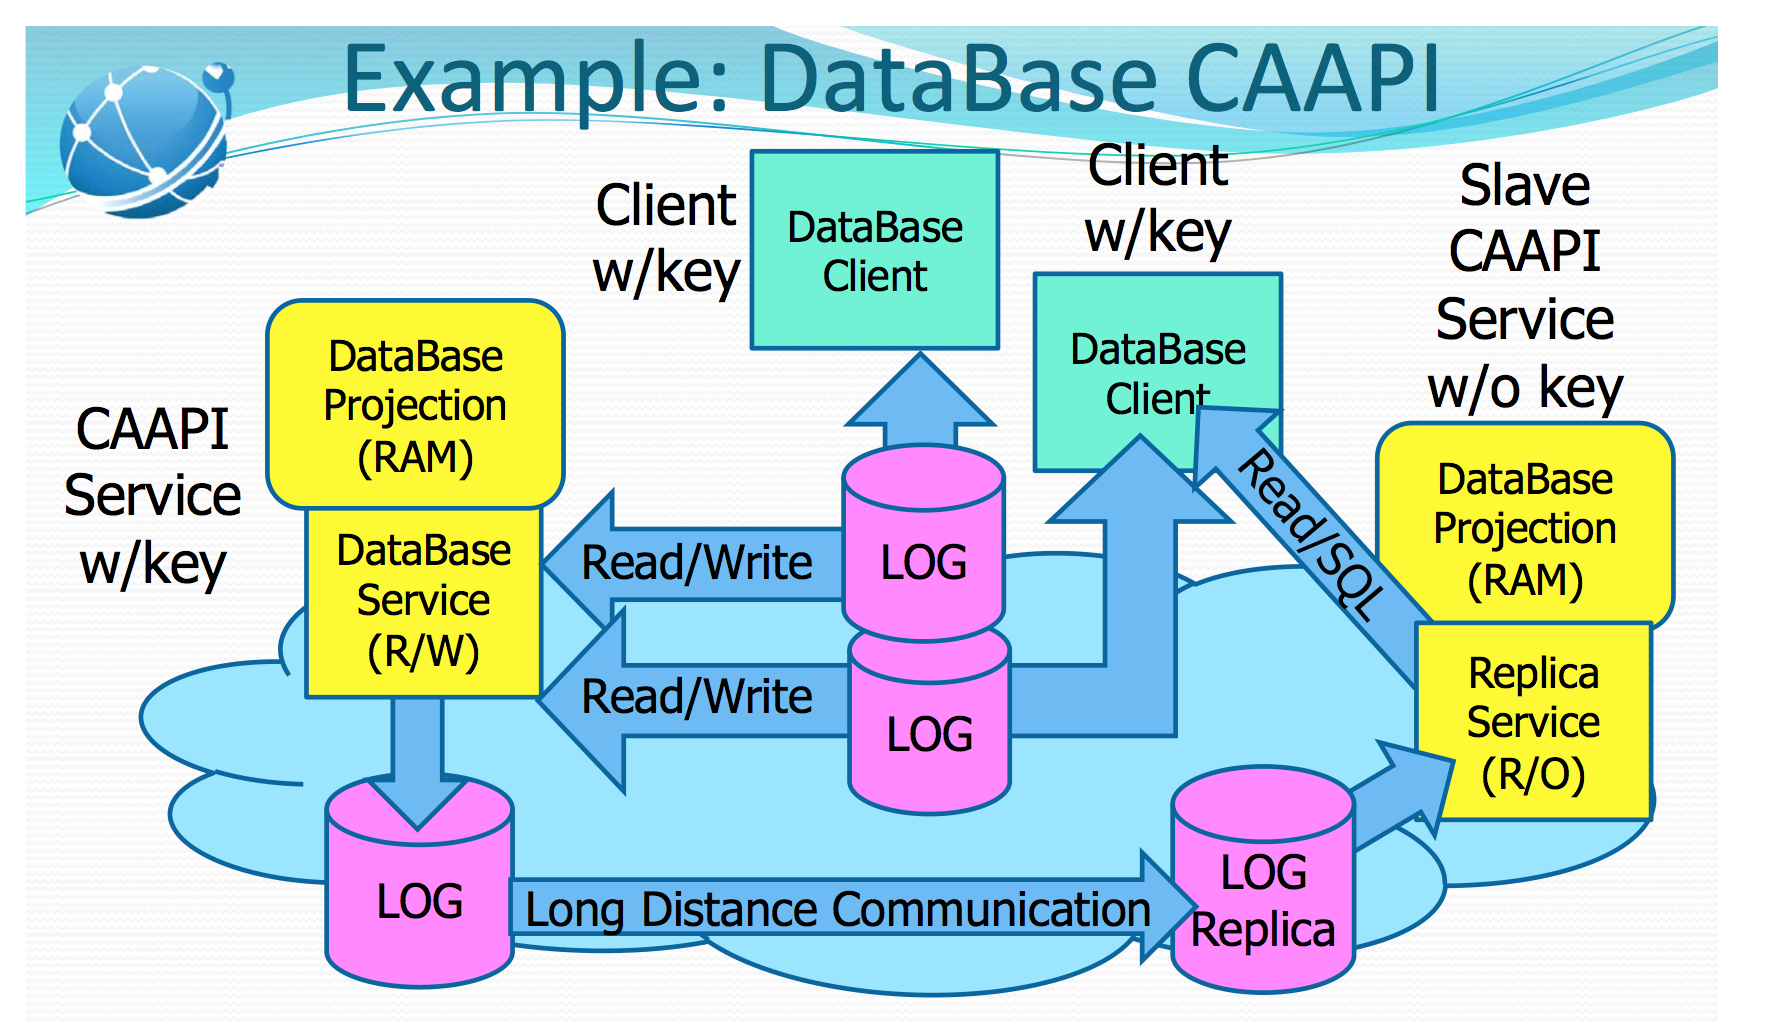
\includegraphics[width=3.5in]{Images/Database_CAAPI.png}
  \end{center}

  \caption{\small Spanner's TrueTime interface. Image from Table 1 of \cite{corbett_spanner:_2012}. Note that t is a timestamp }
  \label{TrueTime}
\end{figure}



\begin{figure}[!b]
  \begin{center}
    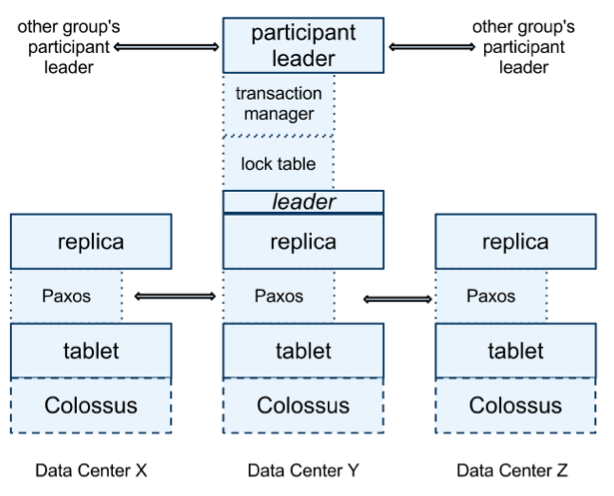
\includegraphics[width=3.5in]{Images/Spanner_Arch.png}
  \end{center}

  \caption{\small Spanner's Architecture. Image from Figure 2 of \cite{corbett_spanner:_2012} }
  \label{Spanner_Arch}
\end{figure}

\section{Background}

Tribune's primary role is to enforce database semantics on a multi-writer log. We chose the semantics of Google Spanner's read write transactions \cite{corbett_spanner:_2012} because Spanner provides a time-based external consistency guarantee and works at a global scale. External consistency establishes the invariant that if transaction A commits before transaction B begins as observed from the outside world, timestamp associated with transaction B in the database must be later than than A's timestamp. Spanner achieves this invariant through a combination of two phase locking within a Paxos group, time-aware two-phase commit between Paxos groups, and precise implementation of the TrueTime API as shown in Figure~\ref{TrueTime}. TrueTime establishes an ordering between timestamps that reflects error in clock synchronization, i.e. it is unknown whether a timestamp proceeds another unless the difference in the timestamps exceeds the known upper bound on the offset between clocks.

Spanner's high level architecture, shown in Figure~\ref{Spanner_Arch}, shares components and terminology with Chubby  \cite{chandra_paxos_2007}, Megastore \cite{baker_megastore:_2011}, and BigTable \cite{chang_bigtable:_2008}, all Google projects as well. In Spanner, the tablets that are associated with a particular data model run on a set of replicas in the same Paxos group. The primary responsibility of the Paxos leader is to replicate the state of writes that go through it across the group. The leader also acts as a bottleneck for all read write transactions, which allows it to maintain a lock table that reflects the status of transactions currently in flight. Clients that want to perform read write transactions must acquire locks through two phase commit, and deadlocks are prevented with wound wait \cite{wound_wait}. When a read write transaction needs to commit across paxos groups (a "distributed transaction"), one paxos leader steps up for the role of participant leader and runs a transaction manager to organize the two-phase commit. Spanner also supports read only transactions and read transactions (the two are actually distinct types in Spanner) that can be performed at any replica without going through the paxos leader.




\subsection{Time Synchronization}
Spanner uses a global network of atomic and gps clocks to achieve time synchronization. An advantage of establishing very accurate clocks with very low drift is that very little communication is needed to preserve synchrony. IEEE 1588, the Precision Time Protocol \cite{ratzel_toward_2012} presents an alternative, ip based mechanism to achieve synchronization on the order of microseconds across a wired local area network. Truetime is used in spanner to determine when to pick timestamps for transactions in two-phase commit and how long to hold locks after committing within a paxos group.  Note that without any kind of synchronization between clients, relativity makes it impossible to evaluate external consistency. The definition of external consistency requires that transactions outside the system exist on a shared timeline (because they must be comparable) which implies some way to compare times at two locations, whether quantitative or logical \cite{lamport_time_1978}.


\subsection{Consensus Algorithms and Durability}

Consensus algorithms like Paxos \cite{Lamport_paxos} and Byzantine Agreement \cite{lamport_byzantine_1982} can be used to build a state machine with an unambiguous history across distributed, faulty machines. As a consequence, data is unambiguously replicated through the system -- a desirable outcome for a global database that must remain consistent and available in the face of datacenter-wide failures.

Paxos and Byzantine Agreement address different failure modes for a distributed state machine. Byzantine agreement tolerates malicious faults while Paxos protocols assume the entire system is trustworthy. There is however, a performance tradeoff. For a system with 2N + 1 nodes, Paxos consensus allows for N nodes to simultaneously disappear. For a system with 3M + 1 nodes, Byzantine Agreement can tolerant M malicious nodes but requires expensive pairwise communication to achieve consensus.  	

Note that availability, as provided by consensus algorithms,  is not the same as durability \cite{weatherspoon_antiquity:_2007}; the former relates to the presence of a backup-copy of a resource accessible in the short-term, where the latter refers to the capacity to protect data from accidental deletion. Reed-Solomon encoding \cite{Reed-Solomon}  is a good approach for long-term data storage when the top objective is reducing the probability that data will be lost. But for short term data storage, using a consensus algorithm to achieve agreement on the state of a set of replicas is a much faster approach. Perhaps the Reed-Solomon encoding data might be verified by a Byzantine Agreement ring as in \cite{rhea_pond:_2003} but in the short term, other methods become much more practical. As a long-term objective for the GDP, the system ought to achieve a balance between both durable and responsive storage.

Another dimension of durability concerns the transfer of data from volatile to non-volatile memory such that a particular machine can recover from a crash or power outage. Although we didn't implement this part of a database in Tribune, algorithms that address this concern (such as \cite{mohan_aries:_1992} and \cite{sears_segment-based_2009} ) are well known in the literature and are applied in most mature databases.

\subsection{Routing in the GDP}
Data must be routed to Tribune in the GDP through an overlay network. Oceanstore used Tapestry \cite{zhao_tapestry_2004}, although a distributed hash table approach such as Chord \cite{stoica_chord:_2003} or Bamboo \cite{rhea_handling_2003} for routing. A project is currently underway in the GDP to efficiently route to the opaque identifiers that signify the location of a log server or a CAAPI.

\begin{figure}[!b]
  \begin{center}
    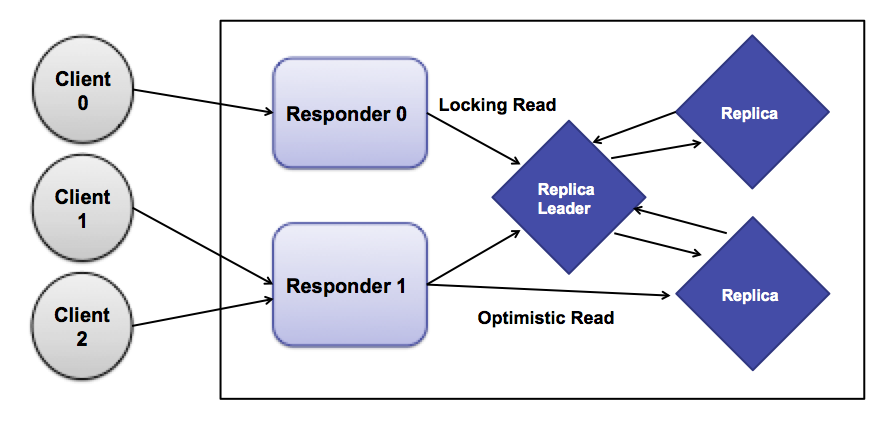
\includegraphics[width=3.5in]{Images/Tribune_Arch.png}
  \end{center}

  \caption{\small Tribune's Architecture. }
  \label{Tribune_Arch}
\end{figure}

\section{Background}


\section{System Architecture}
 \textbf{ARCHITECTURE PICTURES GO HERE!!!}
Our first design of system emulates a simplified version of Google Spanner without any \textbf{ "distributed transaction"}. Because we opt not to handle \textbf{"distributed transactions"}, we do not implement the transaction manager which coordinates two phase commits between different Paxos groups. Our first design of system assumes an one-paxos-group environment so we only implement the lock manager at the leader replica.

The responder receives transactions from client applications. It parses each operation line by line and acquires read locks for all data required for the transaction. The responder buffers writes locally. When all the transaction operation finishes, the responder tries to acquire write locks for the locally modified data. If the attempt turns out successful, the responder will try to commit the transaction at the leader. 

We only implement the necessary components for read-write transactions. So all transactions would go through the leader replica to validate their respective lock leases before committing via paxos protocol. If the validation is successful, the leader would go through all paxos phases and return the final transaction status (abort or commit) back to responder. The responder will return the transaction status back to client apps.

%Below is a diagram for the overall architecture:

\textbf{//then talk about modifications on the first version to incorporate optimistic concurrency control and byzantine agreement}


\section{Algorithms and Implementation}

\textbf{EDIT THIS TO MAKE IT THE RIGHT TENSE}
In this section, we're going to elaborate on the algorithmic part of the project, which is our choices of concurrency control protocol and commit consensus protocol. We did strict two-phase locking and optimistic concurrency for concurrency control. We also did paxos and byzantine agreement for commit consensus protocol. We would explain in detail how we implement four algorithms in our project and compare the tradeoffs in this section. The benchmark results would be in the next section.

\subsection{Programming Tools}

We originally choose to implement Tribune in Java because the project team had familiarity with the language, and we felt a strongly typed, garbage collecting, object oriented language would reduce the frequency of programming errors in development. Java is known to perform "stop the world" garbage collection, in which execution periodically halts in all threads for 10s of milliseconds, but considering the low precision of our ultimate testing environment (three laptops) we decided it was an acceptable penalty given Java's other advantages.

As shown in Figure~\ref{Tribune_Arch}, client processes need to establish a connection with Responders, and Responders must communicate with Replicas, likely all across a network. Early on we experimented with basic java socket IO, but we realized we would have to repetitively implement the same programming idiom of a server that handles the connection and a parser thread that is responsible for reading a custom defined language of intended commands to be called on the receiving object. A little investigation found that this functionality was already available in the Java Remote Method Invocation framework \cite{Pitt:2001:JRM:558733},  so we chose to use it instead of building a similar system from scratch.

However, RMI was not a perfect solution. The RMI server that is started for each registered object does not use a thread pool; it simply forks off a new thread whenever it gets a connection. The Sun implementation of RMI exposes a parameter for the number of TCP connections that can be ongoing at once, but this doesn't limit the number of worker threads that can be alive in the system at a given time. Therefore with a sufficiently large number of clients, spawning an arbitrarily large number of threads the RMI server may be ill-conditioned. Switching to SEDA \cite{welsh_seda:_2001} for future work, would alleviate this problem, but significantly change our programming model.

RMI also presents a naming problem. Surprisingly, RMI does not support a remote rmiregistry where objects can be found directly by registration name. A remote object may only be registered on a local rmiregistry server with a name of the form "\textless{}ip address of host machine\textgreater{}/\textless{}registration name\textgreater{}".  Since our performance evaluation was performed on machines without static ip addresses, we potentially faced an addressing nightmare where the ip address of remote object s would change sporadically. To address this issue, we implemented a naming service over RMI we called Remote Registry, that maps a "\textless{}registration name\textgreater{}" to a full network-ready string of the form "//\textless{}ip address of host machine\textgreater{}/\textless{}registration name\textgreater{}". With Remote Registry we could publish not only the location of an object when its ip address changed, but also the availability of resources during initialization.

\subsection{Initalization}

\subsection{Strict Two-Phase Locking}
\begin{lstlisting}
// Hello.java
import javax.swing.JApplet;
import java.awt.Graphics;

public class Hello extends JApplet {
    public void paintComponent(Graphics g) {
        g.drawString("Hello, world!", 65, 95);
    }    
}
\end{lstlisting}

\subsection{Optimistic Concurrency Control}
Subsubsection text here.

\subsection{Initialization}

\subsection{Pseudo Paxos vs Pseudo Byzantine Agreement}

We had to deal first-hand with a non-obvious implementation detail that arises in the practical implementation of Paxos: out-of-date replicas. We took inspiration from Chubby's solution to the problem  \cite{chandra_paxos_2007} by using sequence numbers to catch a replica back up to the current state of the system when possible. It would be impractical to maintain a permanent map between paxos sequence numbers and changes to the database, so instead we truncate the log at a fixed distance in the past. If a replica is further behind than the end of the log, it asks for a snapshot of the current state of the system from the leader, and achieves up-to-date status.
  
Also, we considered using Raft \cite{ongaro_search_2014} as an alternative to Paxos
We implement the 

\subsection{Remote Method Invocation}

\section{Experiments and Results}
Subsubsection text here.

\section{Future Work}

Spanner-style semantics concerning time are most certainly not the only option for a CAAPI in the GDP. PTIDES \cite{zou_execution_2009} provides both an execution model and a simulation environment for time-aware computation. Rather than dealing with transactions, PTIDES determines the execution of atomic events and enforces that sensor-to-actuator deadlines are met. As an advantage of tight time synchronization and atomic events, PTIDES can define a deterministic time-ordered merge between two input streams by simply waiting out the clock uncertainty before writing. This policy guarantees no future event could be timestamped further in the past than the written value.

Reconsidering our implementation choices now the project is complete, THREADS ARE EVIL






\section{Acknowledgements}
Thanks to Dr. Patricia Derler for her input on Spanner and time synchronization. Also thanks to Prof. John Kubiatowicz for numerous discussions about the GDP and CAAPIs.

\bibliographystyle{abbrv}
\bibliography{My_Library}



\end{document}



